\documentclass[../exploring-pagerank.tex]{subfiles}

\begin{document}
    \begin{figure}
        \centering
        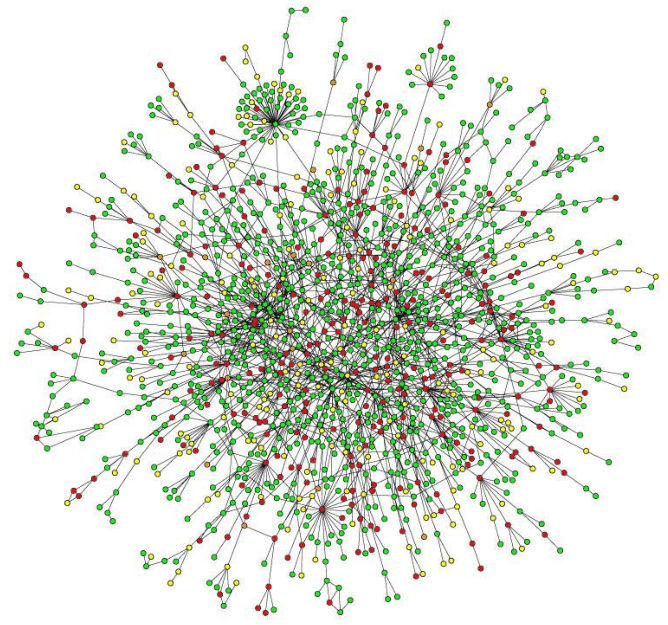
\includegraphics[scale=1.8]{scale-free-network}
        \caption{A Scale-Free Network (Yeast Proteome) \cite{wangKineticConformationalCharacterization}}
        \label{fig:scale-free}
    \end{figure}
    \subsection{Near-Reducibility}
    Consider a Markov chain given by $P=\begin{bsmallmatrix} 1 & 0 \\ 0 & 1 \end{bsmallmatrix}$. The chain is fully reducible, and equivalently, the underlying graph is disconnected. Clearly, $P$ will only have eigenvalue 1 with multiplicity 2. Suppose now we have a chain with $P'=\begin{bsmallmatrix} 1 - \epsilon_1  & \epsilon_1 \\ \epsilon_2 & 1 - \epsilon_2 \end{bsmallmatrix}$, for $\epsilon \in (1,0)$. Thus, the spectrum $\sigma(P') =P' \{ 1, 1-\epsilon_1 - \epsilon_2 \}$. 
    
    Considering the canonical form of reducibility in Equation \eqref{eqn:reducible}, we see that an irreducible Markov chain with subdominant eigenvalue $\lambda_2 \approx 1$ will be nearly reducible. However, the existence of such a subdominant eigenvalue is not by itself sufficient for near-reducibility. Nearly-reducible Markov chains have strong interactions within their clusters, but relatively weak interactions between clusters.\footnote{The formal study of clustering in Markov chains is a well-developed field much better understood through the probabalistic convergence theorem , which we have eschewed here for a linear-algebraic approach.} Note that powerful analysis of graph clustering and subdominant eigenvalues can be done through the graph Laplacian, but we will not expound that tool here.
    
    \subsection{Scale-Free Networks}
    In 1959, Erdős and Rényi proposed generating random graphs by considering a Poisson distribution over the out-degree of vertices. In such a random graph (also called an exponential network), most nodes share a similar number of out-links, and there are very few nodes that deviate from this mean. A random network is thus very democratic and has a steep bell curve. Most natural networks, however, do not follow a random structure. 
    \begin{figure}
        \centering
        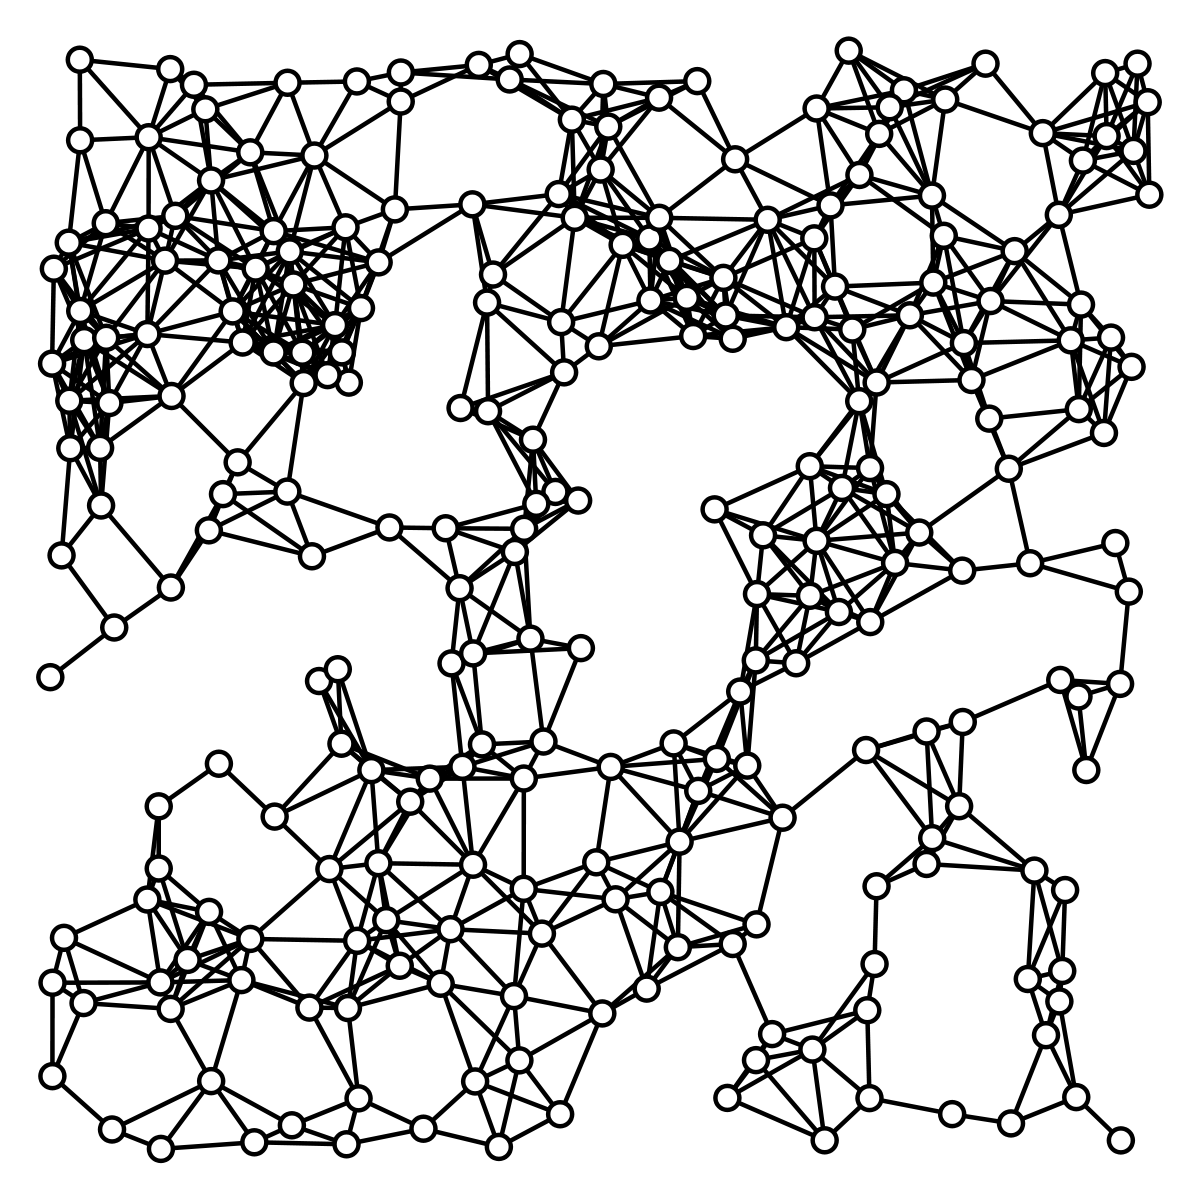
\includegraphics[scale=0.15]{random-graph}
        \caption{A Random Graph \cite{RandomGeometricGraph}}
        \label{fig:random}
    \end{figure}
    Consider Figure \ref{fig:scale-free}, which maps the partial proteome of a yeast. The red nodes, which denote proteins most essential for life, tend to bind together clusters of proteins of lesser importance. Note our use of the term \textit{importance} here. If we only had the proteome graph, sans color, we would likely be able to determine which proteins were most ``important'' for life by computing a spectral rank like the PageRank. Indeed, we have assumed from the start that the most connected nodes are the most important nodes. In fact, HITS -- another spectral rank developed at IBM contemporaneously with PageRank -- makes the pursuit  more explicit by splitting Web pages into hubs and authorities and using the more complex impredicative heuristic that good hubs link to good authorities and vice versa. In a random graph, however, such a definition of importance breaks down.
    
    A music theorist analyzes a piece of classical music by first determining what chords are most important -- that is, what chords are most tonally connected to other chords. However, an atonal piece by Schönberg defies such straightforward analysis; due to the random tonality of the twelve-tone system -- similar to an Erdős-Rényi random graph -- we cannot easily determine which chords are more ``important'' than others.\footnote{This perhaps gives insight into why Schönberg abhored the label \textit{atonal} and much preferred to call his music \textit{pan-tonal}.} They mostly sound alike to our tonal ears, except for a few chance progressions that give a fleeting sense of tonality. Morphing one chord of Schönberg would not much impact the flow of his music, but we can imagine the havoc of omitting a dominant chord of Mozart.
    
    Networks such as these follow a power law. The probability that a node has $k$ outlinks is proportional to $\frac{1}{k^\gamma}$, for some power $\gamma$. Although most nodes have only a few links to others, a few have thousands. Removing just these most important nodes, the hubs, can catastrophically fragment the network into its isolated components disrupt the network. These networks also reveal a beautiful fractal structure; thus, we call them scale-free networks. Sociologists have long known of these networks. The Erdős number and the ``six degrees of Kevin Bacon'' work because a few people are highly connected; they bridge groups of people who would otherwise be unrelated. Though these nodes may be few, they are quite powerful. Income distribution in Western countries can be similarly modeled with a scale-free network. Note that scale-free networks will also be very reducible, as they have strong interactions within their clusters but relatively weak interactions among them.
    
    Both the physical and logical Internet have been shown to be scale-free networks. The Internet is thus highly resilient to random attacks, but destroying just about 3\% of hubs -- the most highly connected ones -- would be enough to fragment the Internet into dozens of isolated components \cite{barabasiNetworkScienceScaleFree}. This suggests that even the large SCC of Figure \ref{fig:web} is not terribly strong against a targeted attacks. By contrast, the strongly-connected components of a random graph would be quite strong, as a random graph has redundancy almost everywhere and thus cannot encode much information.
    
    As we have seen, only scale-free networks have a sufficiently heterogeneous structure to permit a meaningful spectral importance rank. Thus, Markov chains over scale-free networks will have a subdominant eigenvalue quite close to 1. However, the reducibility of these Markov chains thus yields an irony: the very structure that enables a spectral ranking also hampers its calculation. Although the teleportation adjustment ensured the primitivity of the Google matrix, it still tends to leave the dampened Web only weakly irreducible -- that is, nearly reducible. 

    \subsection{Damping Factor}
    Recall $\alpha$, the damping factor used in Equation \eqref{eqn:google_matrix}. This probability $\alpha$ controls the fidelity of the model to the raw Web structure. As $\alpha \to 1$, the Google matrix becomes more nearly reducible, its subdominant eigenvalue $\lambda \to 1$, and the power method converges ever more slowly. Moreover, as $\alpha \to 1$, the limiting distribution becomes far more sensitive -- both in terms of importance score and the consequent PageRanks -- to link changes even within minor clusters; further approaching 1 magnifies these effects. We can explore these results more by analyzing the vector derivative $\frac{d\pi(\alpha)}{d\alpha}$, but we will not do so here.
    
    We learn in \cite{haveliwalaSecondEigenvalueGoogle} that a stochastic matrix $S$ with $\sigma_S = \{ 1, \lambda_2, \lambda_3, \cdots, \lambda_n \}$ gives a Google matrix with $\sigma_G = \alpha\sigma_S = \{ \alpha, \alpha\lambda_2, \alpha\lambda_3, \cdots, \alpha\lambda_n \}$. From this, we see $\lambda_2 \leq \alpha$ for the Google matrix. Thus, the power method converges at the rate which $\alpha^k \to 0$ as $k$ grows. In \cite{brinPageRankCitationRanking1998}, PageRank's authors With $\alpha = 0.85$, Google's formulation of the power method converges within a thousandth by approximately 50 iterations. Note that the power method scales well to immense datasets like the Web graph -- it is an essentially linear algorithm that requires at most 100 iterations to converge satisfactorily to rank all pages on the indexed Web.
\end{document}